%
% $RCSfile: introduction.tex,v $
%
% Copyright (c) 2005-2006. Christian Heller. All rights reserved.
%
% Permission is granted to copy, distribute and/or modify this document
% under the terms of the GNU Free Documentation License, Version 1.1 or
% any later version published by the Free Software Foundation; with no
% Invariant Sections, with no Front-Cover Texts and with no Back-Cover
% Texts. A copy of the license is included in the section entitled
% "GNU Free Documentation License".
%
% http://www.cybop.net
% - Cybernetics Oriented Programming -
%
% http://www.resmedicinae.org
% - Information in Medicine -
%
% Version: $Revision: 1.1 $ $Date: 2006-01-03 08:21:45 $ $Author: christian $
% Authors: Christian Heller <christian.heller@tuxtax.de>
%

\section{Introduction}
\label{introduction_heading}

Sometimes, describing the easy things is the most difficult. And most of the
time, it seems easier to copy existing concepts than to investigate new, but
possibly more intuitive solutions. The work described in this document tried to
question traditional concepts of software design and to correct or simplify
these by applying new ideas stemming from other scientific disciplines. It thus
wants to contribute to a better knowledge modelling.

The initially observed discrepancies belong to software engineering processes
(abstraction gaps), to the physical architecture (misleading tiers) as well as
the logical architecture (modelling mistakes) of systems. They are explained
following.

%
% $RCSfile$
%
% Copyright (c) 2005-2006. Christian Heller. All rights reserved.
%
% Permission is granted to copy, distribute and/or modify this document
% under the terms of the GNU Free Documentation License, Version 1.1 or
% any later version published by the Free Software Foundation; with no
% Invariant Sections, with no Front-Cover Texts and with no Back-Cover
% Texts. A copy of the license is included in the section entitled
% "GNU Free Documentation License".
%
% http://www.cybop.net
% - Cybernetics Oriented Programming -
%
% http://www.resmedicinae.org
% - Information in Medicine -
%
% Version: $Revision$ $Date$ $Author$
% Authors: Christian Heller <christian.heller@tuxtax.de>
%

\subsection{Abstraction Gaps}
\label{abstraction_gaps_heading}

Software has to be developed in a creative process called
\emph{Software Engineering Process} (SEP) or \emph{Methodology} (figure
\ref{gaps_figure}).

\begin{figure}[htb]
    \begin{center}
        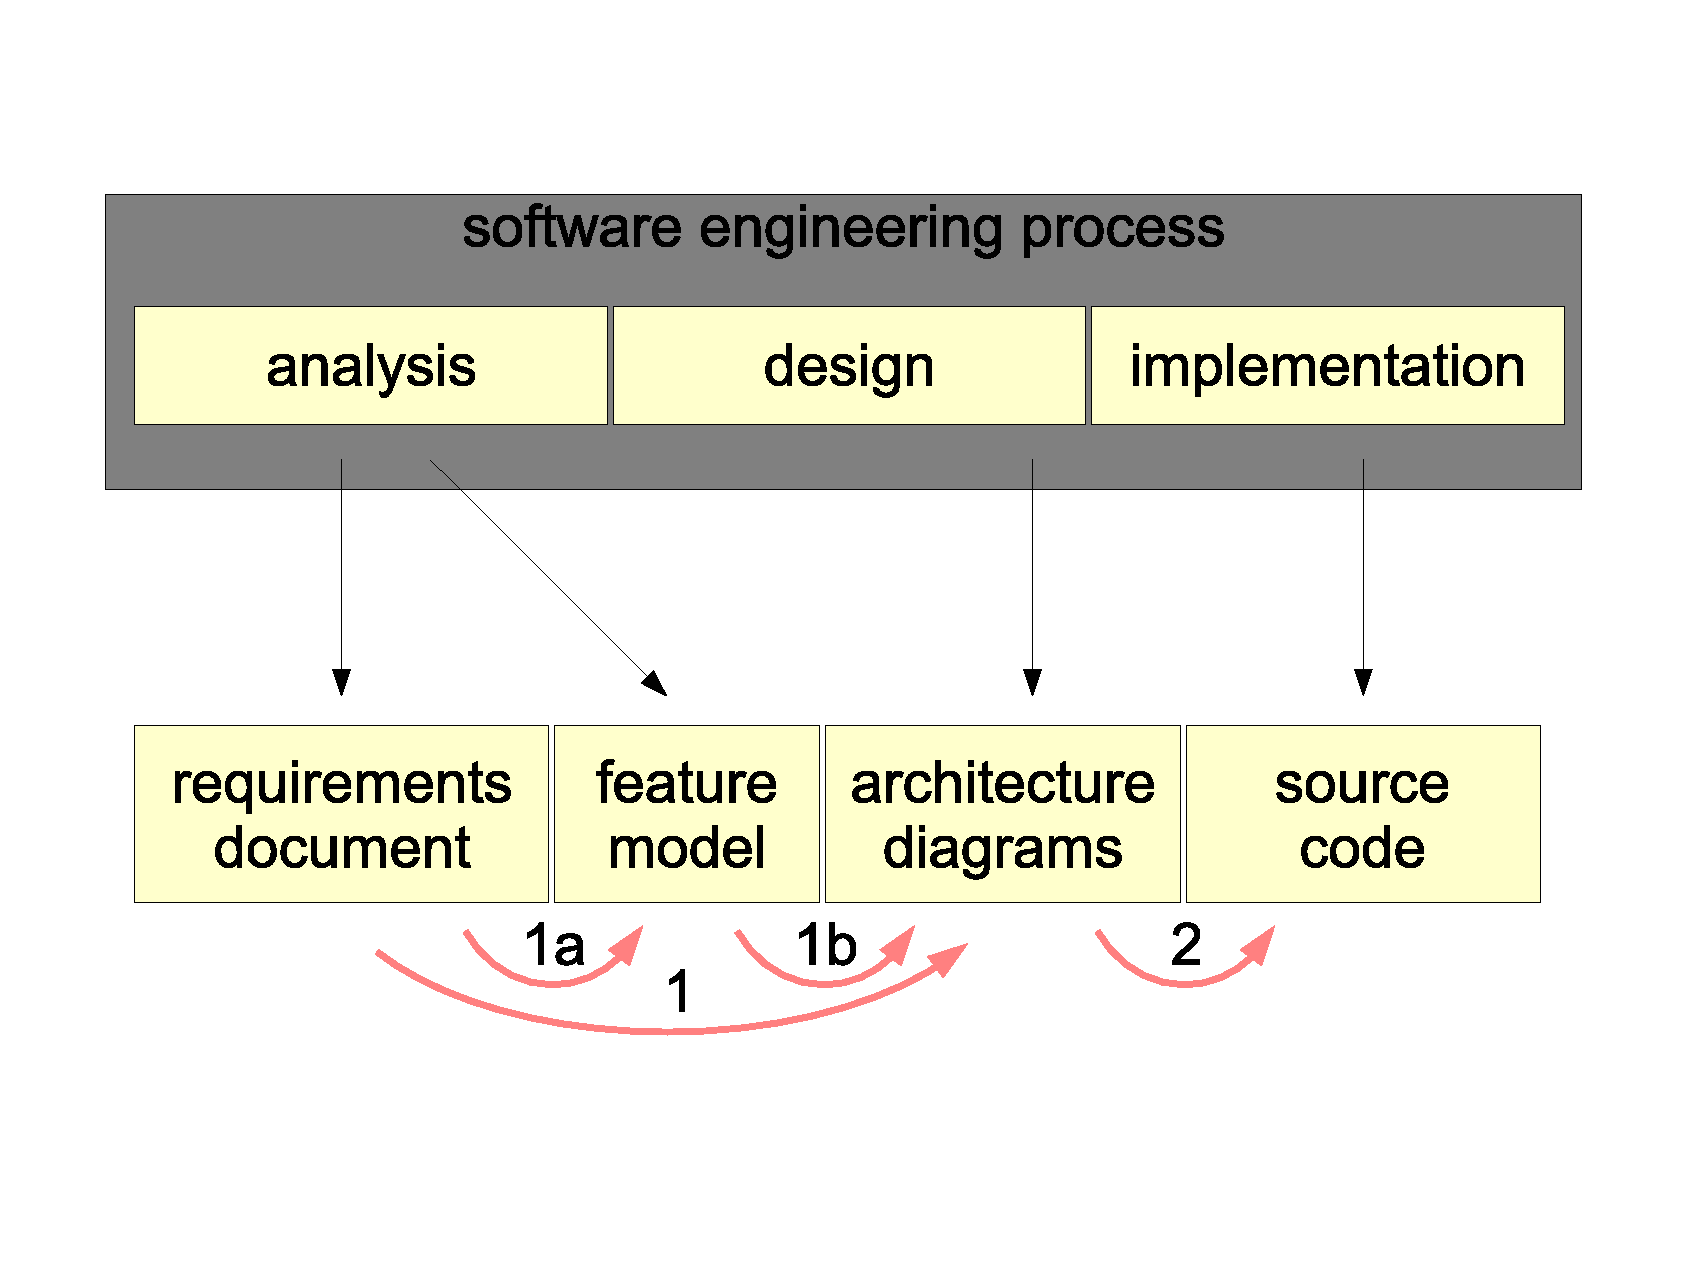
\includegraphics[scale=0.2]{vector/gaps.eps}
        \caption{Abstraction Gaps}
        \label{gaps_figure}
    \end{center}
\end{figure}

Different forms of SEP exist: \emph{Waterfall}, \emph{Iterative},
\emph{Extreme Programming} (XP) and \emph{Agile Programming}. But every
project, consciously or not, follows a SEP that sooner-or-later, in one form or
the other, goes through three common phases: \emph{Analysis}, \emph{Design} and
\emph{Implementation}. Each phase creates its own model of what is to be
abstracted in software and it is the differences in exactly these models that
often cause complications.

A previous article \cite{heller2004} mentioned the \emph{Requirements Document},
\emph{Feature Model}, \emph{Architecture Diagrams} and \emph{Source Code} as
forms of knowledge abstraction. It also described the following abstraction
gaps (see figure \ref{gaps_figure}) that have to be crossed:

\begin{enumerate}
    \item[1a] Requirements Document/Feature M.
    \item[1b] Feature Model/Architecture Diagr.
    \item[2] Architecture Diagrams/Source Code
\end{enumerate}

By improving the \emph{Traceability} between requirements and the architecture,
feature models (known from system family/ product line engineering) contribute
to minimising gap 1. Together with architecture diagrams, they ease
communication between stakeholders in the SEP, because of their human-readable
form and implementation-independence. But sooner-or-later, also these have to
be transferred into source code, by crossing gap 2.

Bridging or closing these abstraction gaps (sometimes called \emph{Semantic- or
Conceptual Gaps}) is also known as: \textit{achieving higher intentionality}
and remains an unsolved task for software engineering. One aim of the work
described in this article was to contribute to a possible solution, with focus
on \emph{reducing} gap 2, existing between a designed architecture and the
implemented code.

%
% $RCSfile$
%
% Copyright (c) 2005-2006. Christian Heller. All rights reserved.
%
% Permission is granted to copy, distribute and/or modify this document
% under the terms of the GNU Free Documentation License, Version 1.1 or
% any later version published by the Free Software Foundation; with no
% Invariant Sections, with no Front-Cover Texts and with no Back-Cover
% Texts. A copy of the license is included in the section entitled
% "GNU Free Documentation License".
%
% http://www.cybop.net
% - Cybernetics Oriented Programming -
%
% http://www.resmedicinae.org
% - Information in Medicine -
%
% Version: $Revision$ $Date$ $Author$
% Authors: Christian Heller <christian.heller@tuxtax.de>
%

\subsection{Misleading Tiers}
\label{misleading_tiers_heading}

When distinguishing human- and technical systems, the kinds of
\emph{Communication} are:

\begin{itemize}
    \item[-] Human $\leftrightarrow$ Human
    \item[-] Human $\leftrightarrow$ Computer
    \item[-] Computer $\leftrightarrow$ Computer
\end{itemize}

Each of these relies on different techniques, transport mechanisms, languages
(protocols) and so on. But the general principle after which communication
works, is always the same -- no matter whether technical \emph{Computer}
systems or their biological prototype, the \emph{Human Being}, are considered:
Information is \emph{received}, \emph{stored}, \emph{processed} and \emph{sent}.
Despite these common characteristics, today's \emph{Information Technology}
(IT) environments \cite{hellerkunze} treat communication between a computer
system and a human being differently than that \emph{among} computer systems.

\begin{figure}[ht]
    \begin{center}
        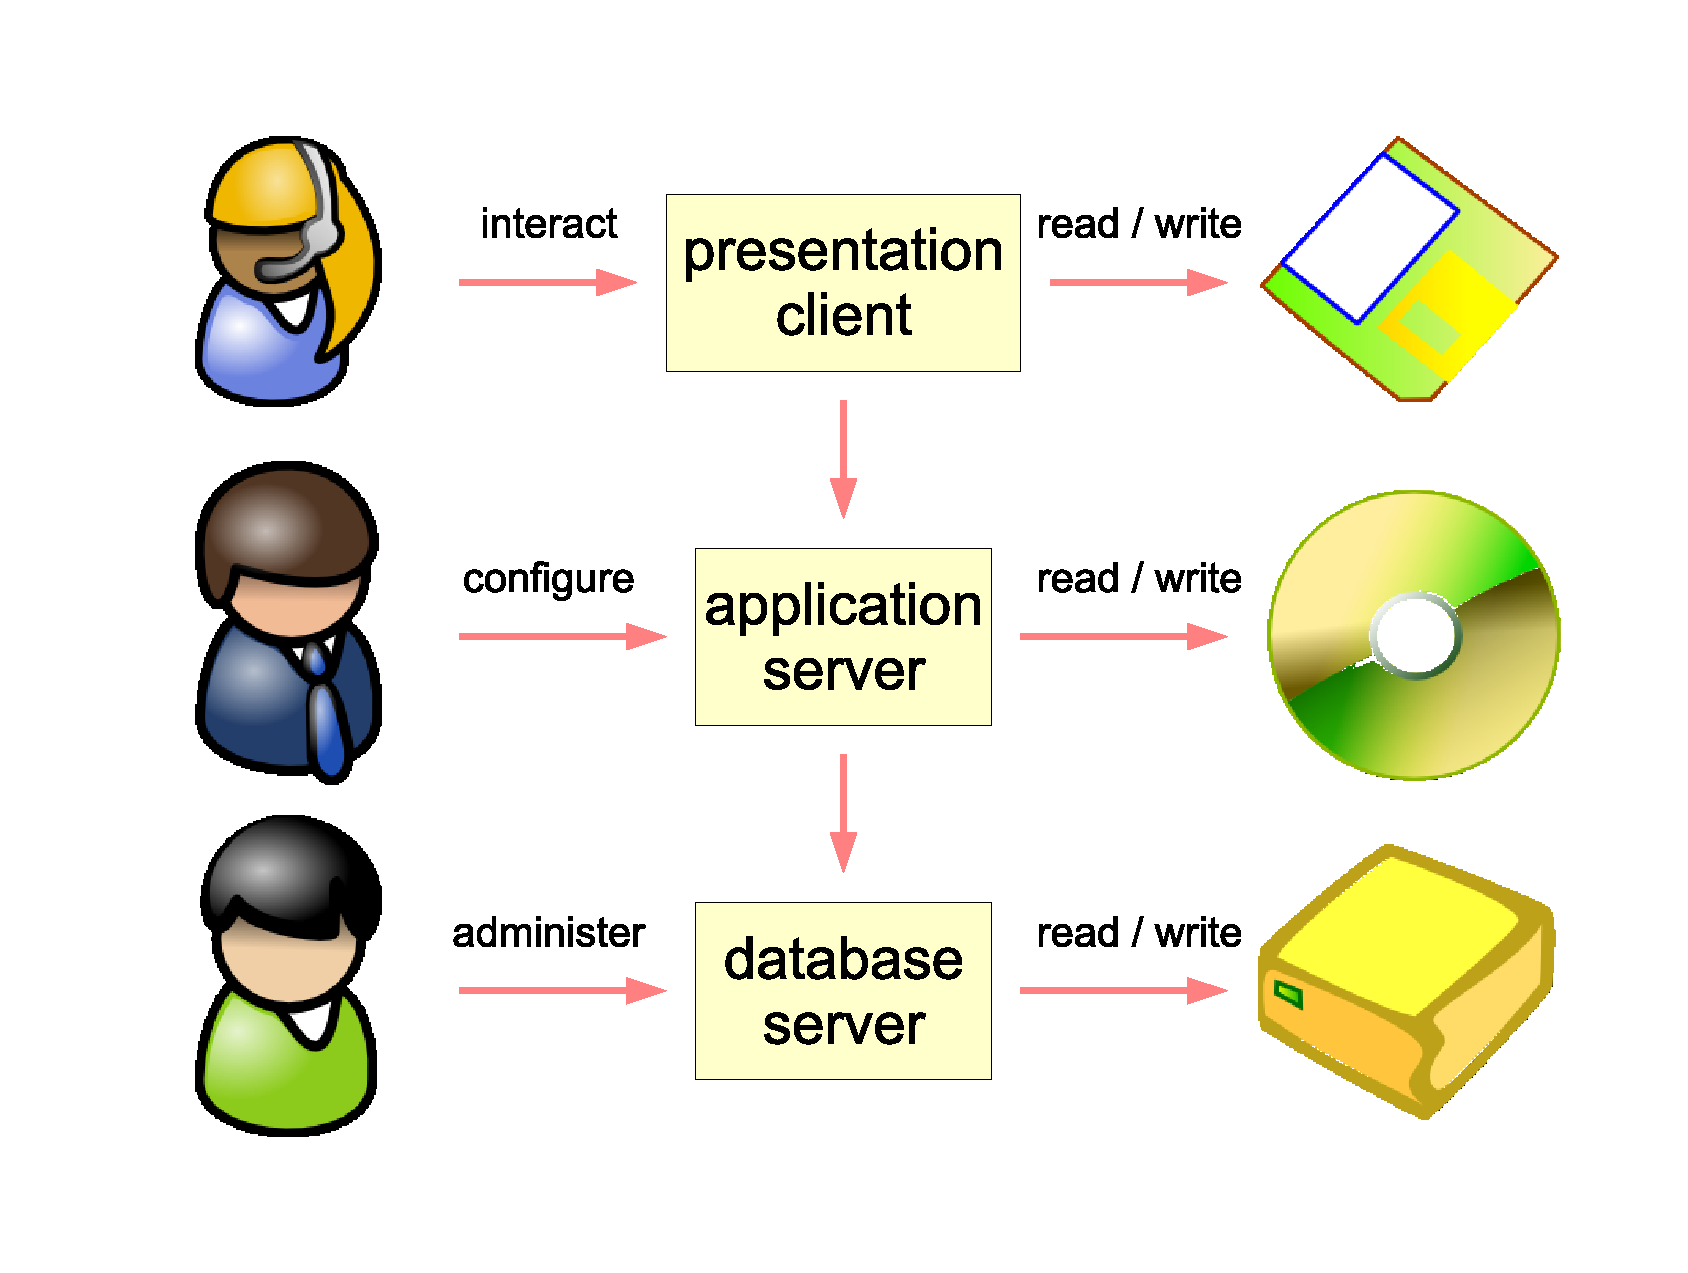
\includegraphics[scale=0.2]{vector/misleading.eps}
        \caption{Universal Communication}
        \label{misleading_figure}
    \end{center}
\end{figure}

Figure \ref{misleading_figure} shows a three-tier environment: tier 1 represents
the \emph{Presentation Layer}; tier 2 stands for the \emph{Application Layer};
tier 3 is the \emph{Database (DB) Layer}. Typical synonyms are, in this order:
\emph{Frontend}, \emph{Business Logic} and \emph{Backend}. The tiers (layers)
serve two needs: connect different locations and share work load (\emph{Scaling}).
However, the split into tiers of that kind raises two illusions:

\begin{enumerate}
    \item \emph{Users only interact with clients}
    \item \emph{Persistent data are stored in DB only}
\end{enumerate}

Many IT architectures, or at least their illustrations, neglect the fact that
in reality \emph{all} systems need a \emph{User Interface} (UI), for at least
being administered by humans, and \emph{almost} all systems, even
\emph{Database Management Systems} (DBMS) themselves, store some of their
persistent data outside a database, for example locally available configuration
information. This is not necessarily a problem for the IT environment as such,
but it is for the internal architecture of software systems. Special solutions
have to deal with frontend (UI framework), business logic (domain patterns) and
backend (data mapping), and often additional mechanisms for local and remote
communication. The serious differences in these design solutions are one root
of well-known problems like multi- directional inter-dependencies between system
parts, that make software difficult to develop and hard to maintain.

One aim of the work described in this article was to investigate possibilities
for a \emph{unification} of communication paradigms, that is high-level design
paradigms rather than low-level protocols, in order to architect software in a
way that allows the computer system it runs on to communicate \emph{universally}.

%
% $RCSfile: modelling_mistakes.tex,v $
%
% Copyright (C) 2002-2008. Christian Heller.
%
% Permission is granted to copy, distribute and/or modify this document
% under the terms of the GNU Free Documentation License, Version 1.1 or
% any later version published by the Free Software Foundation; with no
% Invariant Sections, with no Front-Cover Texts and with no Back-Cover
% Texts. A copy of the license is included in the section entitled
% "GNU Free Documentation License".
%
% http://www.cybop.net
% - Cybernetics Oriented Programming -
%
% http://www.resmedicinae.org
% - Information in Medicine -
%
% Version: $Revision: 1.1 $ $Date: 2008-08-19 20:41:07 $ $Author: christian $
% Authors: Christian Heller <christian.heller@tuxtax.de>
%

\section{Modelling Mistakes}
\label{modelling_mistakes_heading}
\index{Modelling Mistakes}

While the previous chapters elaborated on \emph{Software Engineering Processes}
(SEP) (chapter \ref{software_engineering_process_heading}) and the
\emph{Physical Architecture} of an \emph{Information Technology} (IT)
environment (chapter \ref{physical_architecture_heading}), the sections of this
chapter discussed state-of-the-art solutions for designing and implementing the
\emph{Logical Architecture} of software systems, that is their inner structure.

Computers can be controlled by \emph{Software}. It contains the instructions
after which a computer is run. Instructions can be grouped into levels of
growing abstraction, starting from low-level \emph{Digital Logic}, implemented
in hardware, up to higher-level \emph{Problem Oriented Languages} (POL). The
borders between hardware and software are fluent. Initially, it is up to the
computer constructor to decide whether functionality gets burned into hardware
or coded into software.

A set of computer instructions is known as \emph{Program}; the language a
computer program is written in is known as \emph{Programming Language}. While
for early application systems, it was acceptable to write programs directly in
\emph{Machine-} or \emph{Assembly Language}, later tasks required languages
that were easier and faster to program. A palette of programming languages and
-paradigms was introduced in section \ref{paradigm_and_language_heading}.

The more complex software requirements became, the better solutions had to be
found to cope with them. Unfortunately, the complexity of the requirements is
often targeted with equally complex design- and implementation techniques,
leading to dependencies and high coupling within a system. A whole variety of
such techniques, more or less complex, exists today and this chapter tried to
investigate a rather big percentage of them, mentioning their advantages but
also trying to identify disadvantages. To the investigated concepts belong:

\begin{itemize}
    \item[-] Structure and Procedure; Class and Inheritance (section \ref{paradigm_and_language_heading})
    \item[-] Pattern and Framework (section \ref{pattern_heading})
    \item[-] Component and Concern; Agent with Knowledge Base (section \ref{component_oriented_programming_heading})
    \item[-] Application and Domain; Model generated into Code (section \ref{domain_engineering_heading})
    \item[-] Date and Rule (section \ref{knowledge_engineering_heading})
    \item[-] Terminology and Ontology; Archetype and Dual Model (section \ref{conceptual_network_heading})
\end{itemize}

Some of the identified disadvantages are already addressed and improved by
existing technologies. The inflexible \emph{Static Typing} (section
\ref{system_programming_heading}), for instance, can be avoided with
\emph{Typeless Programming} (section \ref{typeless_programming_heading}).
However, there remains a number of design problems to be solved, the main ones
of which are listed following:

\begin{itemize}
    \item[-] Unpredictable behaviour due to container inheritance
        (section \ref{falsifying_polymorphism_heading})
    \item[-] Differing communication patterns due to wrong models
        (section \ref{architectural_heading})
    \item[-] Bidirectional dependencies due to bad patterns
        (section \ref{bidirectional_dependency_heading})
    \item[-] Global data access due to static methods
        (section \ref{global_access_heading})
    \item[-] Redundant code or spread functionality due to concerns
        (section \ref{spread_functionality_heading})
    \item[-] Provision of a model-only approach to software development
        (section \ref{model_and_code_heading})
    \item[-] Finding of a universal schema for knowledge representation
        (section \ref{dual_model_approach_heading})
\end{itemize}

Many of these are caused by \emph{Modelling Mistakes} that will only turn out
to be mistakes while being compared with inter-disciplinary ideas in later
chapters (part \ref{contribution_heading}). One aim of this work is to improve
software development by offering solutions to these problems. Yet instead of
further complicating software design and -implementation, it tries to bethink
on the elementary principle of programming, namely the: \textit{Abstraction of
states and logic in form of static knowledge, in order to dynamically control a
computer system}. More on this in the following chapter.

